\documentclass[aspectratio=169]{beamer}

\usetheme{Boadilla}
\usefonttheme{professionalfonts}
\setbeamertemplate{navigation symbols}{}
\setbeamertemplate{itemize items}[circle]
\setbeamertemplate{enumerate items}[default]
\setbeamertemplate{headline}{}

\usepackage[utf8]{inputenc}
\usepackage[T1]{fontenc}
\usepackage{lmodern}
\usepackage{amsmath}
\usepackage{booktabs}
\usepackage{tabularx}
\usepackage{array}
\usepackage{hyperref}
\usepackage[strings]{underscore}
\usepackage{listings}
\usepackage{tikz}
\usetikzlibrary{arrows.meta,positioning,fit,calc,shapes.geometric}
\usepackage{xcolor}

\definecolor{courseblue}{HTML}{12355B}
\definecolor{coursegold}{HTML}{C98A2E}
\definecolor{courseice}{HTML}{EEF3F8}
\definecolor{coursegreen}{HTML}{2F6B4F}
\definecolor{coursegray}{HTML}{4B5563}
\definecolor{codebg}{HTML}{F7F9FC}
\definecolor{codecomment}{HTML}{5E6C84}
\definecolor{codestring}{HTML}{0B6E4F}

\setbeamercolor{palette primary}{bg=courseblue,fg=white}
\setbeamercolor{palette secondary}{bg=coursegold,fg=white}
\setbeamercolor{palette tertiary}{bg=courseblue,fg=white}
\setbeamercolor{palette quaternary}{bg=coursegold,fg=white}
\setbeamercolor{structure}{fg=courseblue}
\setbeamercolor{frametitle}{bg=courseice,fg=courseblue}
\setbeamercolor{title}{fg=courseblue}
\setbeamercolor{block title}{bg=courseblue,fg=white}
\setbeamercolor{block body}{bg=courseice,fg=black}
\setbeamercolor{normal text}{fg=black,bg=white}
\setbeamercolor{alerted text}{fg=coursegold}

\setbeamerfont{footline}{size=\scriptsize}

\setbeamertemplate{footline}{
  \leavevmode
  \hbox{
    \begin{beamercolorbox}[wd=.33\paperwidth,ht=2.8ex,dp=1.2ex,leftskip=0.8em]{palette primary}%
      University of Trieste
    \end{beamercolorbox}%
    \begin{beamercolorbox}[wd=.49\paperwidth,ht=2.8ex,dp=1.2ex,center]{palette tertiary}%
      \coursename{} \textbar{} \coursecode
    \end{beamercolorbox}%
    \begin{beamercolorbox}[wd=.18\paperwidth,ht=2.8ex,dp=1.2ex,rightskip=0.8em plus1fil]{palette secondary}%
      \insertframenumber{} / \inserttotalframenumber
    \end{beamercolorbox}%
  }
}

\hypersetup{
  colorlinks=true,
  linkcolor=courseblue,
  urlcolor=coursegreen
}

\lstdefinestyle{coursepython}{
  language=Python,
  basicstyle=\ttfamily\footnotesize,
  keywordstyle=\color{courseblue}\bfseries,
  commentstyle=\color{codecomment}\itshape,
  stringstyle=\color{codestring},
  showstringspaces=false,
  columns=fullflexible,
  keepspaces=true,
  frame=single,
  framerule=0.6pt,
  rulecolor=\color{courseblue},
  backgroundcolor=\color{codebg},
  xleftmargin=0.4em,
  xrightmargin=0.4em,
  aboveskip=0.4em,
  belowskip=0.2em
}

\newcommand{\coursename}{Data-driven Systems Engineering}
\newcommand{\coursecode}{440MI / 305SM}
\newcommand{\coursefooter}{}

\newcommand{\learninggoals}[1]{
  \begin{block}{Learning goals}
  #1
  \end{block}
}

\newcommand{\repoactivity}[1]{
  \begin{block}{Repo activity}
  #1
  \end{block}
}

\newcommand{\readinglist}[1]{
  \begin{block}{Papers and materials}
  {\footnotesize #1}
  \end{block}
}

\newcommand{\coursecontextframe}[5]{
  \begin{frame}{Course Map and Running Cases}
  \centering
  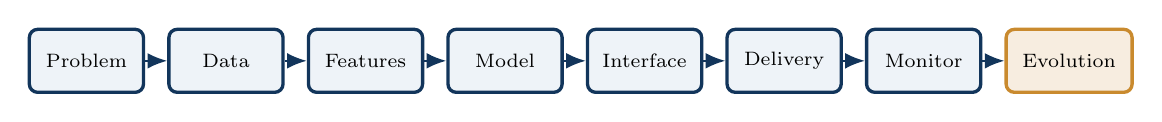
\begin{tikzpicture}[node distance=0.28cm]
  \node[flowbox, minimum width=1.45cm, minimum height=0.8cm] (problem) {\scriptsize Problem};
  \node[flowbox, minimum width=1.45cm, minimum height=0.8cm, right=of problem] (data) {\scriptsize Data};
  \node[flowbox, minimum width=1.45cm, minimum height=0.8cm, right=of data] (features) {\scriptsize Features};
  \node[flowbox, minimum width=1.45cm, minimum height=0.8cm, right=of features] (model) {\scriptsize Model};
  \node[flowbox, minimum width=1.45cm, minimum height=0.8cm, right=of model] (interface) {\scriptsize Interface};
  \node[flowbox, minimum width=1.45cm, minimum height=0.8cm, right=of interface] (delivery) {\scriptsize Delivery};
  \node[flowbox, minimum width=1.45cm, minimum height=0.8cm, right=of delivery] (monitor) {\scriptsize Monitor};
  \node[accentbox, minimum width=1.6cm, minimum height=0.8cm, right=of monitor] (evolution) {\scriptsize Evolution};
  \foreach \a/\b in {problem/data,data/features,features/model,model/interface,interface/delivery,delivery/monitor,monitor/evolution} {
    \draw[arrow] (\a) -- (\b);
  }
  \end{tikzpicture}

  \vspace{0.5em}
  \begin{block}{Today in the course}
  \textbf{Focus:} #1

  \textbf{Bridge:} #2
  \end{block}

  \begin{columns}[T]
  \column{0.48\textwidth}
  \begin{block}{Fraud case}
  {\footnotesize #3}
  \end{block}
  \column{0.48\textwidth}
  \begin{block}{Pasteurization case}
  {\footnotesize #4}
  \end{block}
  \end{columns}

  \vspace{0.3em}
  {\footnotesize \textbf{Course thread:} #5}
  \coursefooter
  \end{frame}
}

\newcommand{\classclosingframe}[4]{
  \begin{frame}{From This Class to the Next}
  \begin{block}{What stays with us}
  #1
  \end{block}

  \begin{columns}[T]
  \column{0.48\textwidth}
  \begin{block}{Project use}
  {\footnotesize #2}
  \end{block}
  \column{0.48\textwidth}
  \begin{block}{Next connection}
  {\footnotesize #3}
  \end{block}
  \end{columns}

  \vspace{0.3em}
  {\footnotesize \textbf{Course thread:} #4}
  \coursefooter
  \end{frame}
}

\tikzset{
  flowbox/.style={
    rounded corners=3pt,
    draw=courseblue,
    fill=courseice,
    very thick,
    minimum width=2.2cm,
    minimum height=0.9cm,
    align=center,
    font=\small
  },
  accentbox/.style={
    rounded corners=3pt,
    draw=coursegold,
    fill=coursegold!15,
    very thick,
    minimum width=2.2cm,
    minimum height=0.9cm,
    align=center,
    font=\small
  },
  arrow/.style={
    -{Latex[length=2.5mm,width=2mm]},
    thick,
    draw=courseblue
  }
}


\title{Class 8: Experiment Tracking and Model Tuning}
\author{\coursename}
\date{}

\begin{document}

\frame{\titlepage \coursefooter}

\begin{frame}{Agenda}
\begin{itemize}
\item Why experiment tracking is part of engineering, not only analysis.
\item Designing experiments before running them.
\item What must be logged to compare models fairly.
\item Tuning strategies and when to use each one.
\item Repository context: Neptune-style experimentation and fraud-model comparison.
\item How experiment records support MLOps later.
\end{itemize}
\coursefooter
\end{frame}

\begin{frame}{Why this class fills an important gap}
\learninggoals{
\begin{itemize}
\item Turn model comparison into a reproducible engineering practice.
\item Connect hyperparameter tuning with logging, provenance, and fair comparison.
\item Prepare students for MLOps workflows where experiments become auditable assets.
\item Distinguish exploration from disciplined experimentation.
\end{itemize}
}
\coursefooter
\end{frame}

\coursecontextframe
{Disciplined experimentation and fair model comparison.}
{This class connects modeling ideas to engineering evidence by making runs, baselines, and provenance comparable.}
{In the fraud case, experiment tracking supports fair comparison across preprocessing choices, model families, and threshold strategies.}
{In the pasteurization case, experiment tracking can compare forecasting variants, online settings, or drift-handling choices without losing context.}
{The thread here is that a good model choice must be explainable, repeatable, and ready for later delivery.}

\begin{frame}{An experiment is a decision-making tool}
\begin{itemize}
\item The purpose of experimentation is not to collect many scores, but to support a credible model choice.
\item Every run should answer a question: does a new feature set help, does a different model family help, or does tuning justify extra complexity?
\item When the question is unclear, experiment tracking becomes a storage system for confusion.
\end{itemize}
\coursefooter
\end{frame}

\begin{frame}{Design the experiment before pressing run}
\begin{itemize}
\item Define the target metric and why it matters operationally.
\item Fix the evaluation protocol before looking at results.
\item Decide which variables are changing and which are held constant.
\item Record what counts as a meaningful improvement.
\end{itemize}
\begin{block}{Examples}
Changing both preprocessing and model family in the same run may be useful, but it makes causal interpretation harder unless the experiment question was framed that way.
\end{block}
\coursefooter
\end{frame}

\begin{frame}{What must be tracked in every experiment}
\begin{itemize}
\item Dataset version or extraction date.
\item Feature pipeline version.
\item Hyperparameters and random seeds.
\item Metrics, confusion matrices, and artifacts.
\item Code commit or notebook snapshot.
\end{itemize}
\coursefooter
\end{frame}

\begin{frame}{Artifacts, lineage, and reproducibility}
\begin{itemize}
\item Metrics alone are insufficient because teams also need the trained artifact, code context, and preprocessing lineage.
\item A useful run can be replayed, audited, and compared months later.
\item Lineage means we can answer: which data, which code, which parameters, and which artifact produced this result?
\end{itemize}
\coursefooter
\end{frame}

\begin{frame}{Why experiment tracking matters}
\begin{itemize}
\item Without metadata, good results become hard to reproduce.
\item Teams need evidence for why one model was selected over another.
\item Tracking helps separate real improvements from accidental differences in preprocessing or data splits.
\item Experiment history becomes valuable once retraining and audits begin.
\end{itemize}
\coursefooter
\end{frame}

\begin{frame}{Repo anchor for this lecture}
\repoactivity{
`notebooks/Class7_Model_Tuning_Neptune.ipynb` gives a natural entry point for discussing experiment metadata, model comparison, and why ad hoc notebook tuning quickly becomes unmanageable.
}
\begin{block}{Better example}
Compare two fraud models with similar AUC but different precision at the operational review threshold.
\end{block}
\coursefooter
\end{frame}

\begin{frame}{What makes a comparison fair?}
\begin{itemize}
\item Same dataset split or same evaluation protocol.
\item Same preprocessing assumptions unless preprocessing is the experiment itself.
\item Metrics chosen to reflect the operational decision.
\item Clear record of training time, latency, artifact size, and maintenance burden.
\end{itemize}
\coursefooter
\end{frame}

\begin{frame}{Common sources of experimental bias}
\begin{itemize}
\item Reusing the test set repeatedly until it becomes part of the tuning loop.
\item Comparing runs produced from different random splits without documenting variance.
\item Mixing notebook state, manual edits, and hidden preprocessing changes.
\item Reporting only the winning run instead of the search process that produced it.
\end{itemize}
\coursefooter
\end{frame}

\begin{frame}{Model search strategies}
\begin{tabularx}{\textwidth}{>{\bfseries}l X}
Strategy & Best use \\
\toprule
Manual tuning & Small problems and pedagogical intuition. \\
Grid search & Small, well-structured search spaces. \\
Random search & Better coverage when many hyperparameters matter unevenly. \\
Bayesian optimization & Expensive models where each run has high cost. \\
\bottomrule
\end{tabularx}
\coursefooter
\end{frame}

\begin{frame}{Baselines matter more than they seem}
\begin{itemize}
\item A tuned model should beat a simple baseline by a meaningful margin.
\item Baselines expose whether the added complexity is actually buying value.
\item They also help students avoid treating hyperparameter search as the first step.
\end{itemize}
\begin{block}{Examples}
Linear regression, a default tree-based model, or a previously deployed model can all serve as strong baselines depending on the task.
\end{block}
\coursefooter
\end{frame}

\begin{frame}[fragile]{Notebook example: defining a search space}
\begin{lstlisting}[style=coursepython]
model = GradientBoostingRegressor(random_state=42)

param_grid = {
    "n_estimators": [100, 200, 300],
    "max_depth": [3, 5, 7],
    "learning_rate": [0.05, 0.1, 0.2],
    "min_samples_split": [2, 5, 10],
}
\end{lstlisting}
\begin{itemize}
\item This follows `notebooks/Class7_Model_Tuning_Neptune.ipynb`.
\item It gives students a realistic example of trade-offs among model complexity, fit time, and predictive gain.
\end{itemize}
\coursefooter
\end{frame}

\begin{frame}[fragile]{Notebook example: tuning and logging}
\begin{lstlisting}[style=coursepython]
grid_search = GridSearchCV(
    estimator=model,
    param_grid=param_grid,
    cv=5,
    scoring="r2",
    n_jobs=-1,
)

grid_search.fit(X_train, y_train)
run["best/parameters"] = grid_search.best_params_
run["best/cv_score"] = grid_search.best_score_
\end{lstlisting}
\begin{itemize}
\item The important idea is not Neptune alone, but the discipline of storing parameters and metrics together.
\item That same pattern later maps naturally to MLflow, Weights \& Biases, or internal experiment registries.
\end{itemize}
\coursefooter
\end{frame}

\begin{frame}{From tuning to model selection}
\begin{itemize}
\item The best validation score is not automatically the best system choice.
\item Sometimes a slightly weaker model is easier to deploy, explain, or monitor.
\item The selected model should align with cost, interpretability, and retraining needs.
\end{itemize}
\coursefooter
\end{frame}

\begin{frame}{From notebook run to governed asset}
\centering
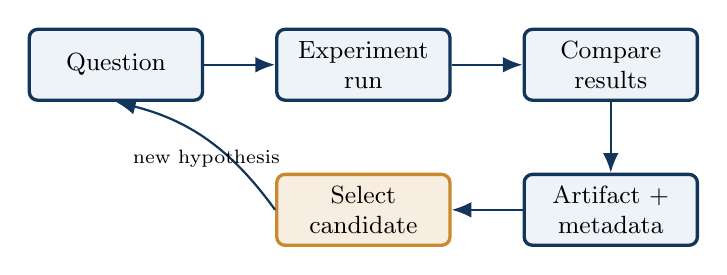
\begin{tikzpicture}[node distance=0.9cm and 0.9cm]
\node[flowbox] (question) {Question};
\node[flowbox, right=of question] (run) {Experiment\\run};
\node[flowbox, right=of run] (compare) {Compare\\results};
\node[flowbox, below=of compare] (artifact) {Artifact +\\metadata};
\node[accentbox, left=of artifact] (select) {Select\\candidate};
\draw[arrow] (question) -- (run);
\draw[arrow] (run) -- (compare);
\draw[arrow] (compare) -- (artifact);
\draw[arrow] (artifact) -- (select);
\draw[arrow, bend right=20] (select.west) to node[below, font=\scriptsize] {new hypothesis} (question.south);
\end{tikzpicture}
\coursefooter
\end{frame}

\begin{frame}{Common tuning mistakes}
\begin{itemize}
\item Tuning on the test set.
\item Comparing runs trained on different preprocessing logic.
\item Reporting only the best metric, not variability or cost.
\item Ignoring class imbalance and threshold behavior.
\item Forgetting that a slightly worse model may be much easier to operate.
\end{itemize}
\coursefooter
\end{frame}

\begin{frame}{What this prepares us for next}
\begin{itemize}
\item Delivery pipelines need stable artifacts and reproducible build inputs.
\item Requirements engineering needs measurable acceptance criteria, not only better scores.
\item Monitoring later depends on knowing which experiment produced the deployed behavior.
\end{itemize}
\coursefooter
\end{frame}

\begin{frame}[fragile]{Notebook example: evaluate and persist the winner}
\begin{lstlisting}[style=coursepython]
best_model = grid_search.best_estimator_
y_pred = best_model.predict(X_test)

run["test/mse"] = mean_squared_error(y_test, y_pred)
run["test/r2"] = r2_score(y_test, y_pred)

joblib.dump(best_model, "best_gb_model.pkl")
run["artifacts/model"].upload("best_gb_model.pkl")
\end{lstlisting}
\begin{itemize}
\item A useful experiment ends with a traceable artifact, not only with a screenshot of the best score.
\item This slide also helps bridge experiment tracking to model registry and deployment topics.
\end{itemize}
\coursefooter
\end{frame}

\begin{frame}{Technology links}
\readinglist{
\href{https://docs.neptune.ai/}{Neptune documentation};\ 
\href{https://mlflow.org/docs/latest/index.html}{MLflow documentation};\ 
\href{https://scikit-learn.org/stable/modules/grid_search.html}{scikit-learn model selection guide};\ 
\href{https://scikit-learn.org/stable/modules/generated/sklearn.model_selection.GridSearchCV.html}{GridSearchCV API}.
}
\coursefooter
\end{frame}

\classclosingframe
{\begin{itemize}
\item A useful experiment records data, configuration, metrics, and artifacts together.
\item Hyperparameter search is valuable only when it is reproducible and comparable.
\item Tracking prevents teams from repeating work or trusting results they cannot explain.
\end{itemize}}
{This gives project teams a disciplined way to compare alternatives, preserve evidence, and package the winning model for later delivery.}
{Class 9 extends that traceability into containers and CI/CD pipelines so experiments can become repeatable releases.}
{Reproducible experimentation is the bridge between exploratory modeling and operational delivery.}

\begin{frame}{Papers and materials}
\readinglist{
\href{https://jmlr.org/papers/volume13/bergstra12a/bergstra12a.pdf}{Bergstra and Bengio (2012), Random Search};\ 
\href{https://proceedings.mlr.press/v28/bergstra13.html}{Bergstra et al. (2013), Hyperopt};\ 
\href{https://docs.neptune.ai/}{Neptune documentation};\ 
\href{https://mlflow.org/docs/latest/index.html}{MLflow documentation}.
}
\coursefooter
\end{frame}

\end{document}
